\documentclass[tikz,border=2pt]{standalone}
\usepackage{pgfplots}
\usetikzlibrary{shapes.geometric, intersections}
\pgfplotsset{compat=1.7}

\begin{document}
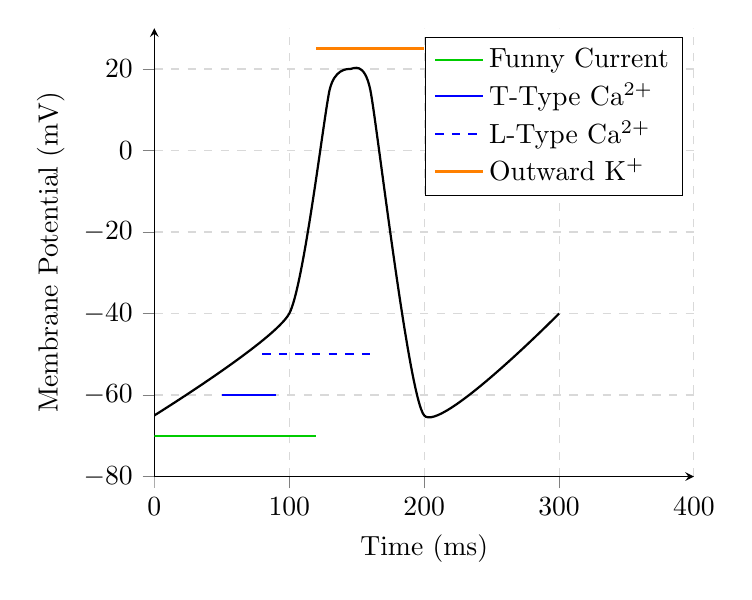
\begin{tikzpicture}

    \begin{axis}[
axis x line=bottom,
  axis y line=left,
	ymin = -80,
	ymax = 30,
	xmin = 0,
xmax = 400,
        grid = major,
        grid style={dashed, gray!30},
	 ylabel near ticks,
	xlabel near ticks,
        xlabel=Time (ms),
        ylabel=Membrane Potential (mV),
        tick align=outside,
        enlargelimits=false,
legend cell align={left}]

\draw[black, thick] plot[smooth,tension=0.3] coordinates { (axis cs: 0,-65) (axis cs: 100,-40) (axis cs: 130,15) (axis cs: 145,20) (axis cs: 160,15) (axis cs: 200,-65) (axis cs: 300,-40)};

\addplot[green!80!black, thick, domain=0:120]{-70};
\addlegendentry{Funny Current};
\addplot[blue, thick, domain=50:90]{-60};
\addlegendentry{T-Type Ca\textsuperscript{2+}};
\addplot[blue,thick,dashed,domain=80:160]{-50};
\addlegendentry{L-Type Ca\textsuperscript{2+}};
\addplot[orange,thick,domain=120:200]{25};
\addlegendentry{Outward K\textsuperscript{+}};




\end{axis}

\end{tikzpicture} 
\end{document}